% Options for packages loaded elsewhere
\PassOptionsToPackage{unicode}{hyperref}
\PassOptionsToPackage{hyphens}{url}
%
\documentclass[
  english,
  man,floatsintext]{apa6}
\title{GenSamp: RESULTS}
\author{Gleb Furman\textsuperscript{1}, James E. Pustejovsky\textsuperscript{2}, \& Elizabeth Tipton\textsuperscript{3}}
\date{}

\usepackage{amsmath,amssymb}
\usepackage{lmodern}
\usepackage{iftex}
\ifPDFTeX
  \usepackage[T1]{fontenc}
  \usepackage[utf8]{inputenc}
  \usepackage{textcomp} % provide euro and other symbols
\else % if luatex or xetex
  \usepackage{unicode-math}
  \defaultfontfeatures{Scale=MatchLowercase}
  \defaultfontfeatures[\rmfamily]{Ligatures=TeX,Scale=1}
\fi
% Use upquote if available, for straight quotes in verbatim environments
\IfFileExists{upquote.sty}{\usepackage{upquote}}{}
\IfFileExists{microtype.sty}{% use microtype if available
  \usepackage[]{microtype}
  \UseMicrotypeSet[protrusion]{basicmath} % disable protrusion for tt fonts
}{}
\makeatletter
\@ifundefined{KOMAClassName}{% if non-KOMA class
  \IfFileExists{parskip.sty}{%
    \usepackage{parskip}
  }{% else
    \setlength{\parindent}{0pt}
    \setlength{\parskip}{6pt plus 2pt minus 1pt}}
}{% if KOMA class
  \KOMAoptions{parskip=half}}
\makeatother
\usepackage{xcolor}
\IfFileExists{xurl.sty}{\usepackage{xurl}}{} % add URL line breaks if available
\IfFileExists{bookmark.sty}{\usepackage{bookmark}}{\usepackage{hyperref}}
\hypersetup{
  pdftitle={GenSamp: RESULTS},
  pdfauthor={Gleb Furman1, James E. Pustejovsky2, \& Elizabeth Tipton3},
  pdflang={en-EN},
  hidelinks,
  pdfcreator={LaTeX via pandoc}}
\urlstyle{same} % disable monospaced font for URLs
\usepackage{graphicx}
\makeatletter
\def\maxwidth{\ifdim\Gin@nat@width>\linewidth\linewidth\else\Gin@nat@width\fi}
\def\maxheight{\ifdim\Gin@nat@height>\textheight\textheight\else\Gin@nat@height\fi}
\makeatother
% Scale images if necessary, so that they will not overflow the page
% margins by default, and it is still possible to overwrite the defaults
% using explicit options in \includegraphics[width, height, ...]{}
\setkeys{Gin}{width=\maxwidth,height=\maxheight,keepaspectratio}
% Set default figure placement to htbp
\makeatletter
\def\fps@figure{htbp}
\makeatother
\setlength{\emergencystretch}{3em} % prevent overfull lines
\providecommand{\tightlist}{%
  \setlength{\itemsep}{0pt}\setlength{\parskip}{0pt}}
\setcounter{secnumdepth}{-\maxdimen} % remove section numbering
% Make \paragraph and \subparagraph free-standing
\ifx\paragraph\undefined\else
  \let\oldparagraph\paragraph
  \renewcommand{\paragraph}[1]{\oldparagraph{#1}\mbox{}}
\fi
\ifx\subparagraph\undefined\else
  \let\oldsubparagraph\subparagraph
  \renewcommand{\subparagraph}[1]{\oldsubparagraph{#1}\mbox{}}
\fi
% Manuscript styling
\usepackage{upgreek}
\captionsetup{font=singlespacing,justification=justified}

% Table formatting
\usepackage{longtable}
\usepackage{lscape}
% \usepackage[counterclockwise]{rotating}   % Landscape page setup for large tables
\usepackage{multirow}		% Table styling
\usepackage{tabularx}		% Control Column width
\usepackage[flushleft]{threeparttable}	% Allows for three part tables with a specified notes section
\usepackage{threeparttablex}            % Lets threeparttable work with longtable

% Create new environments so endfloat can handle them
% \newenvironment{ltable}
%   {\begin{landscape}\centering\begin{threeparttable}}
%   {\end{threeparttable}\end{landscape}}
\newenvironment{lltable}{\begin{landscape}\centering\begin{ThreePartTable}}{\end{ThreePartTable}\end{landscape}}

% Enables adjusting longtable caption width to table width
% Solution found at http://golatex.de/longtable-mit-caption-so-breit-wie-die-tabelle-t15767.html
\makeatletter
\newcommand\LastLTentrywidth{1em}
\newlength\longtablewidth
\setlength{\longtablewidth}{1in}
\newcommand{\getlongtablewidth}{\begingroup \ifcsname LT@\roman{LT@tables}\endcsname \global\longtablewidth=0pt \renewcommand{\LT@entry}[2]{\global\advance\longtablewidth by ##2\relax\gdef\LastLTentrywidth{##2}}\@nameuse{LT@\roman{LT@tables}} \fi \endgroup}

% \setlength{\parindent}{0.5in}
% \setlength{\parskip}{0pt plus 0pt minus 0pt}

% \usepackage{etoolbox}
\makeatletter
\patchcmd{\HyOrg@maketitle}
  {\section{\normalfont\normalsize\abstractname}}
  {\section*{\normalfont\normalsize\abstractname}}
  {}{\typeout{Failed to patch abstract.}}
\patchcmd{\HyOrg@maketitle}
  {\section{\protect\normalfont{\@title}}}
  {\section*{\protect\normalfont{\@title}}}
  {}{\typeout{Failed to patch title.}}
\makeatother
\shorttitle{RESULTS}
\usepackage{csquotes}
\ifXeTeX
  % Load polyglossia as late as possible: uses bidi with RTL langages (e.g. Hebrew, Arabic)
  \usepackage{polyglossia}
  \setmainlanguage[]{english}
\else
  \usepackage[main=english]{babel}
% get rid of language-specific shorthands (see #6817):
\let\LanguageShortHands\languageshorthands
\def\languageshorthands#1{}
\fi
\ifLuaTeX
  \usepackage{selnolig}  % disable illegal ligatures
\fi


\affiliation{\vspace{0.5cm}\textsuperscript{1} University of Texas at Austin\\\textsuperscript{2} University of Wisconsin-Madison\\\textsuperscript{3} Northwestern University}

\begin{document}
\maketitle

\hypertarget{setup}{%
\section{Setup}\label{setup}}

\hypertarget{packages-and-data}{%
\subsection{Packages and Data}\label{packages-and-data}}

\hypertarget{organize-objects}{%
\subsection{Organize Objects}\label{organize-objects}}

\hypertarget{data-summary}{%
\section{Data Summary}\label{data-summary}}

\hypertarget{covaraite-statistics}{%
\subsection{Covaraite Statistics}\label{covaraite-statistics}}

\hypertarget{continuous-variable-distributions}{%
\subsection{Continuous variable distributions}\label{continuous-variable-distributions}}

\begin{verbatim}
## `stat_bin()` using `bins = 30`. Pick better value with `binwidth`.
\end{verbatim}

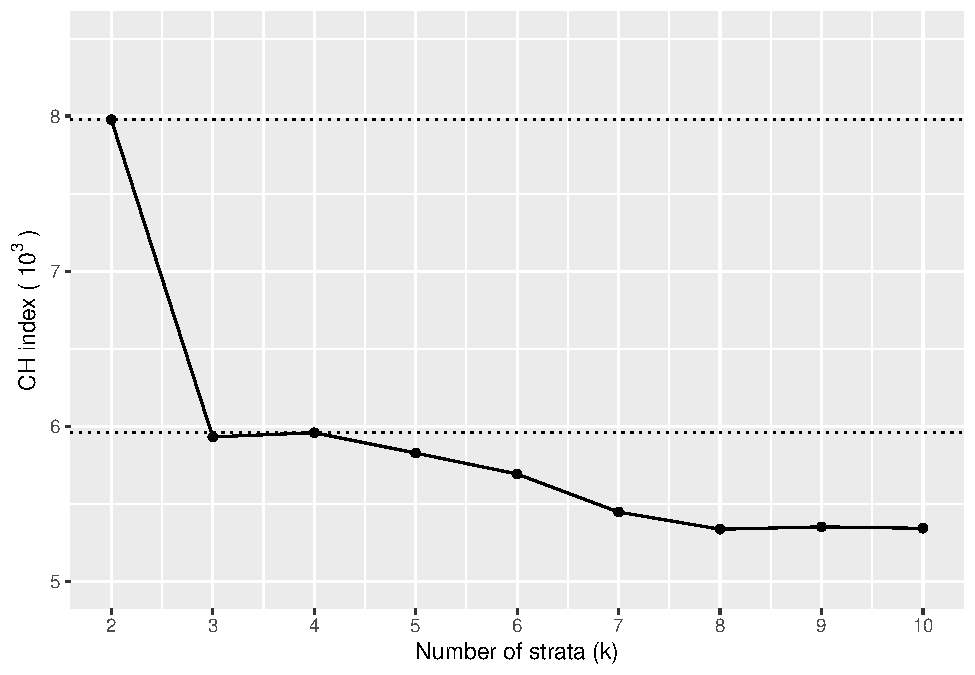
\includegraphics{5---Analysis_files/figure-latex/unnamed-chunk-3-1.pdf}

\hypertarget{methods-summary}{%
\section{Methods Summary}\label{methods-summary}}

\hypertarget{cluster-analysis}{%
\subsection{Cluster Analysis}\label{cluster-analysis}}

\hypertarget{selecting-k}{%
\subsubsection{Selecting k}\label{selecting-k}}

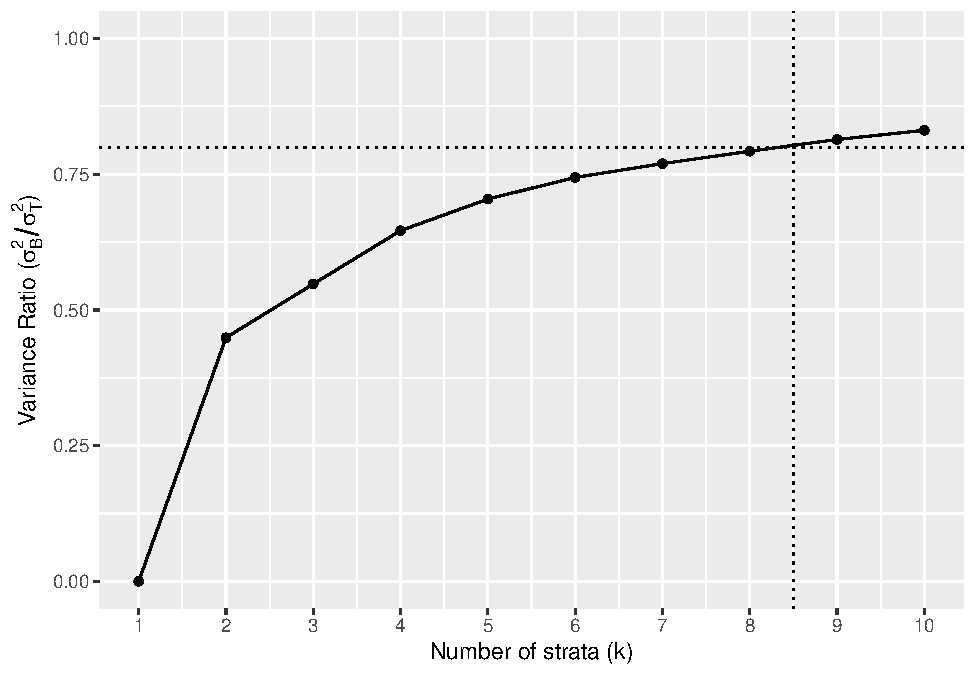
\includegraphics{5---Analysis_files/figure-latex/unnamed-chunk-4-1.pdf}

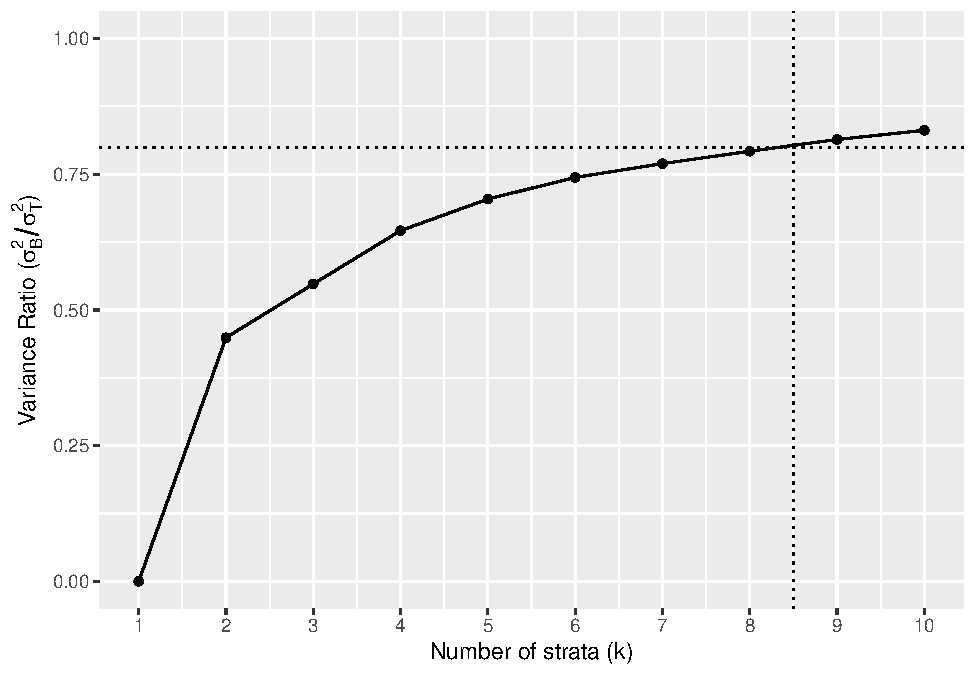
\includegraphics{5---Analysis_files/figure-latex/unnamed-chunk-5-1.pdf}

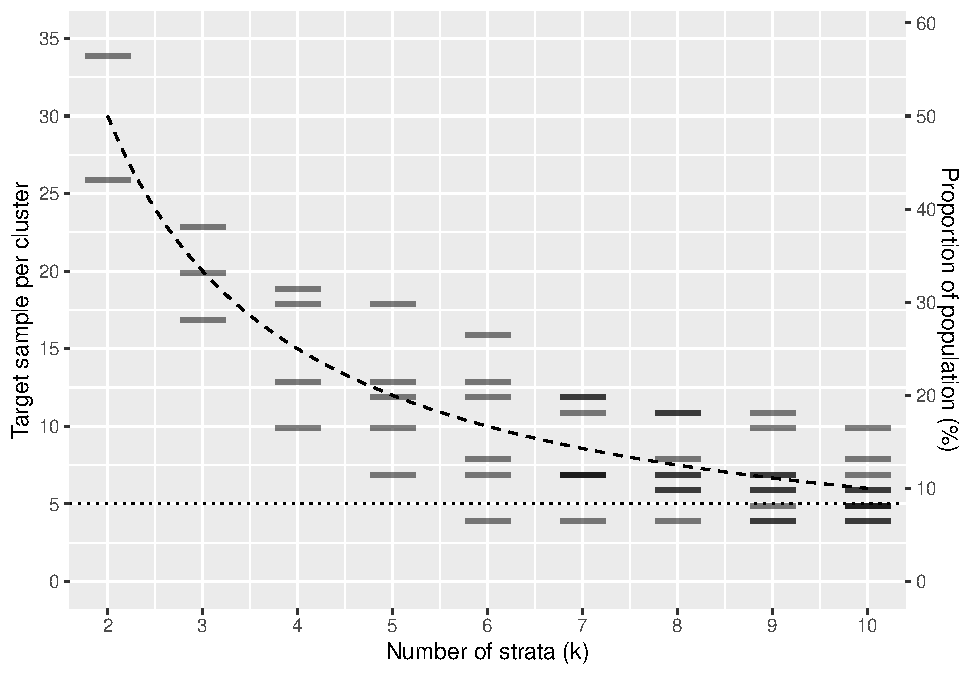
\includegraphics{5---Analysis_files/figure-latex/unnamed-chunk-6-1.pdf}

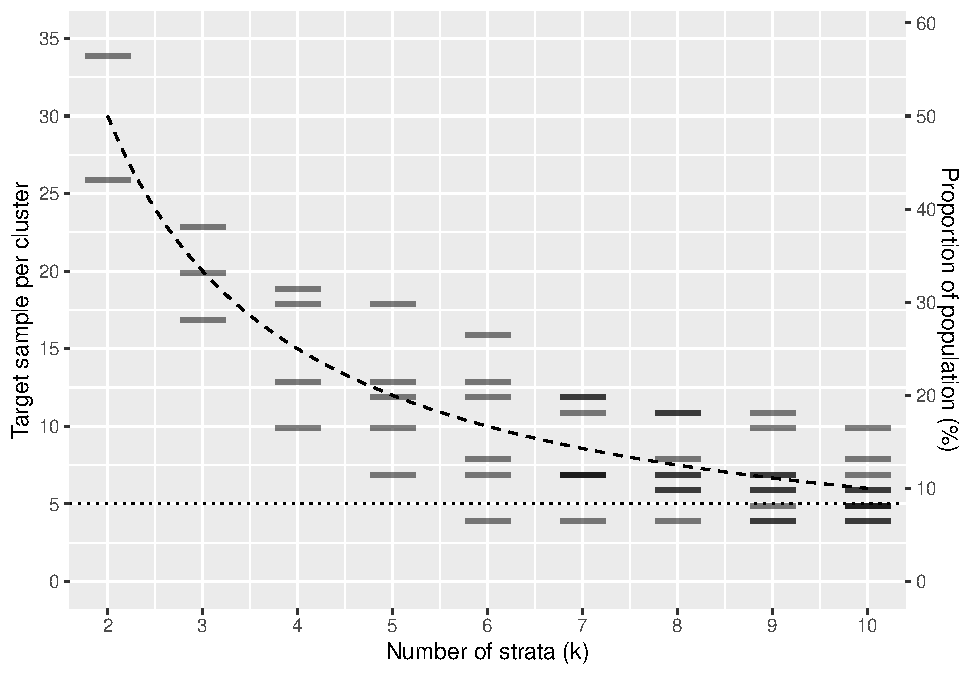
\includegraphics{5---Analysis_files/figure-latex/unnamed-chunk-7-1.pdf}

\begin{verbatim}
## Warning: Using alpha for a discrete variable is not advised.
\end{verbatim}

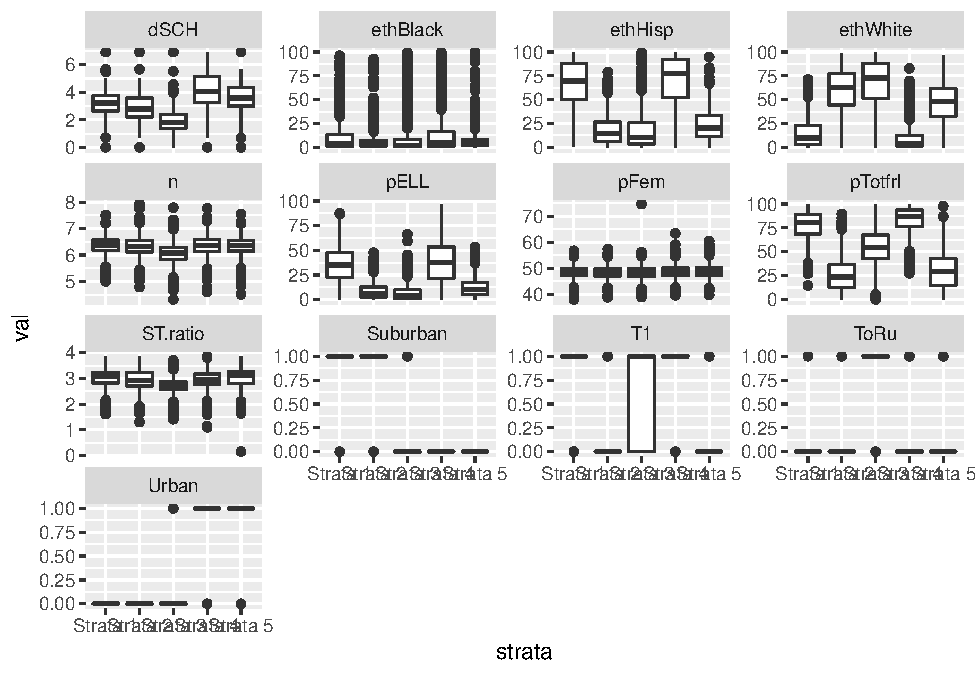
\includegraphics{5---Analysis_files/figure-latex/unnamed-chunk-9-1.pdf}

\hypertarget{variation-explained-by-the-strata}{%
\subsection{Variation explained by the strata}\label{variation-explained-by-the-strata}}

\hypertarget{participation-generating-model}{%
\subsection{Participation Generating Model}\label{participation-generating-model}}

\begin{table}
\centering
\begin{tabular}{l|l|l|l|r}
\hline
Sub & Category & Type & Variables & log\_odds\\
\hline
Status & School Data & Prop & Schoolwide Title I & 0.019\\
\hline
Enrollment & School Data & Mean & School Size & 0.374\\
\hline
Status & Student Data & Mean & Free/Reduced Lunch & 0.081\\
\hline
Urbanicity & School Data & Prop & Urban & 0.433\\
\hline
Urbanicity & School Data & Prop & Suburban & 0.007\\
\hline
Urbanicity & School Data & Prop & Town/Rural & -0.403\\
\hline
Ethnicity & Student Data & Mean & \% White & -0.538\\
\hline
Ethnicity & Student Data & Mean & \% Black & 0.291\\
\hline
Ethnicity & Student Data & Mean & \% Hispanic & 0.395\\
\hline
Gender & Student Data & Mean & \% Female & -0.019\\
\hline
Enrollment & School Data & Mean & Student/Teacher Ratio & -0.101\\
\hline
District & School Data & Mean & District Size & 0.520\\
\hline
Status & Student Data & Mean & English Language Learners & 0.412\\
\hline
\end{tabular}
\end{table}

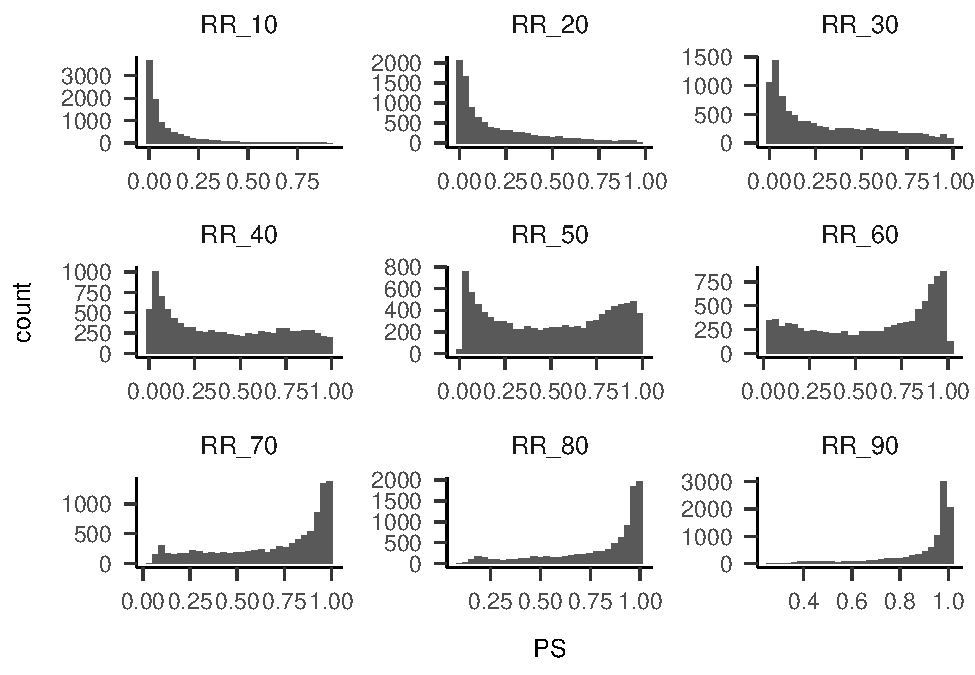
\includegraphics{5---Analysis_files/figure-latex/unnamed-chunk-12-1.pdf}

\begin{figure}
\centering
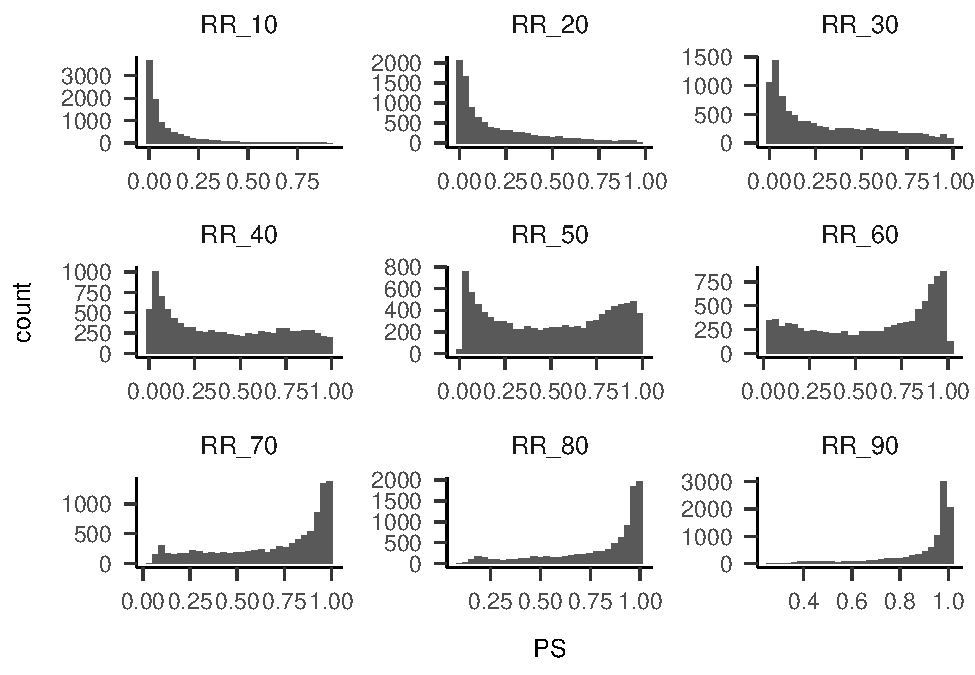
\includegraphics{5---Analysis_files/figure-latex/unnamed-chunk-13-1.pdf}
\caption{\label{fig:unnamed-chunk-13}Distributions of Participation Logits}
\end{figure}

\hypertarget{results}{%
\section{Results}\label{results}}

\hypertarget{generalizability}{%
\subsection{Generalizability}\label{generalizability}}

\hypertarget{b-index}{%
\subsubsection{B Index}\label{b-index}}

\begin{figure}
\centering
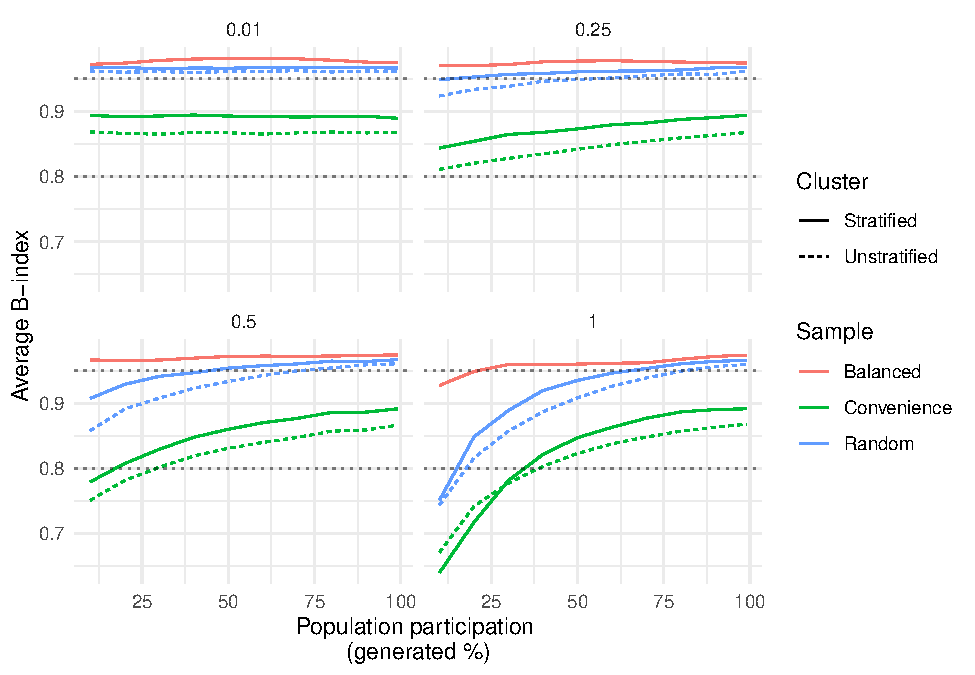
\includegraphics{5---Analysis_files/figure-latex/unnamed-chunk-15-1.pdf}
\caption{\label{fig:unnamed-chunk-15}Averge B-Index}
\end{figure}

\begin{verbatim}
## Note: Using an external vector in selections is ambiguous.
## i Use `all_of(variable)` instead of `variable` to silence this message.
## i See <https://tidyselect.r-lib.org/reference/faq-external-vector.html>.
## This message is displayed once per session.
## Note: Using an external vector in selections is ambiguous.
## i Use `all_of(observations)` instead of `observations` to silence this message.
## i See <https://tidyselect.r-lib.org/reference/faq-external-vector.html>.
## This message is displayed once per session.
\end{verbatim}

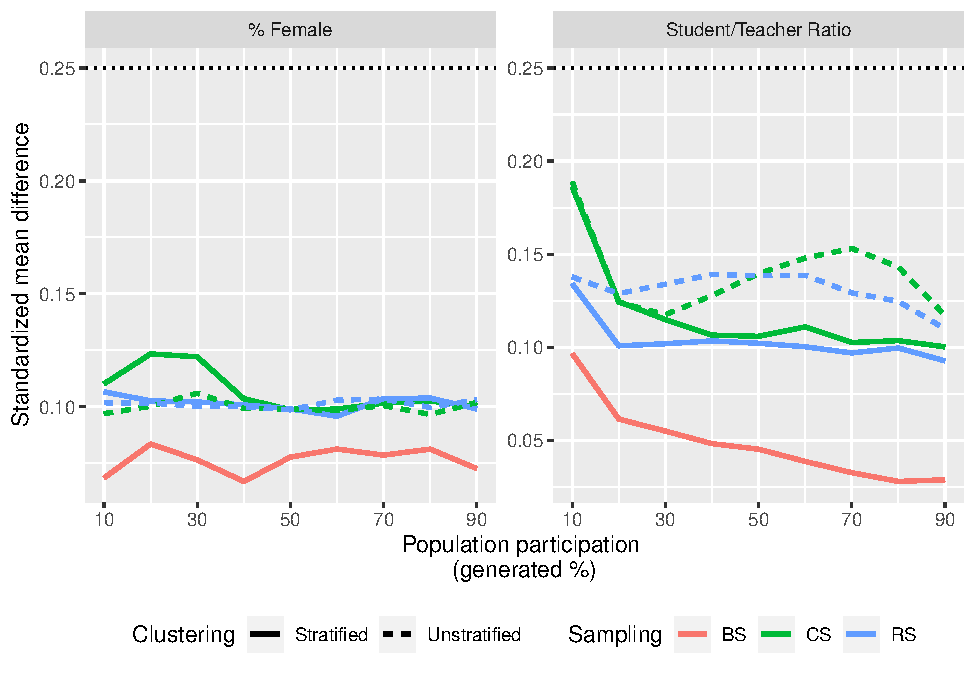
\includegraphics{5---Analysis_files/figure-latex/unnamed-chunk-16-1.pdf}

\hypertarget{standardized-mean-differences}{%
\subsubsection{Standardized mean differences}\label{standardized-mean-differences}}

\hypertarget{group-1}{%
\paragraph{Group 1}\label{group-1}}

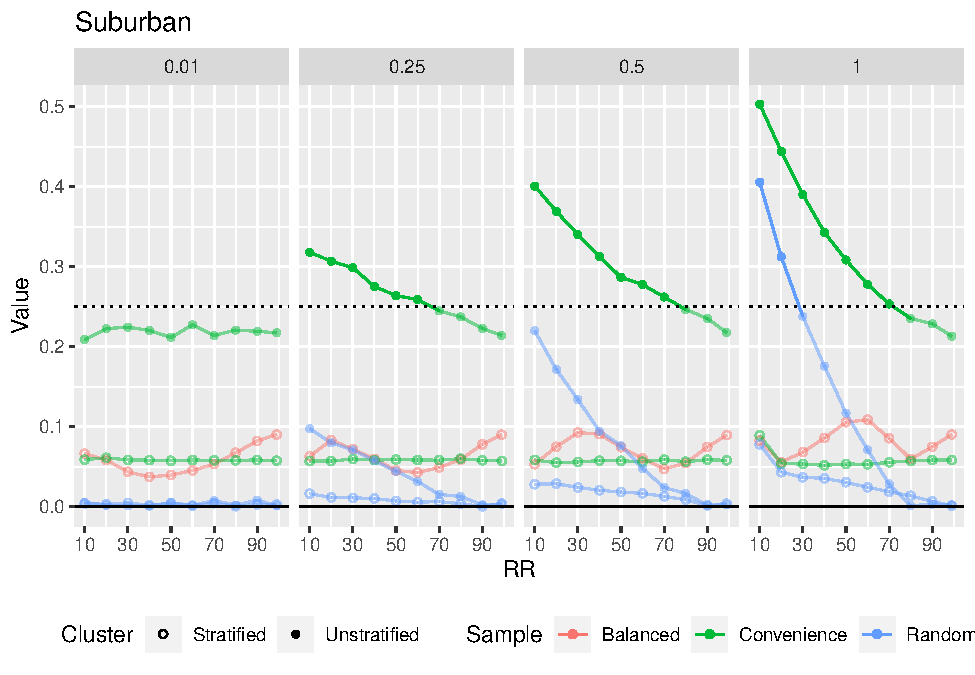
\includegraphics{5---Analysis_files/figure-latex/unnamed-chunk-18-1.pdf} 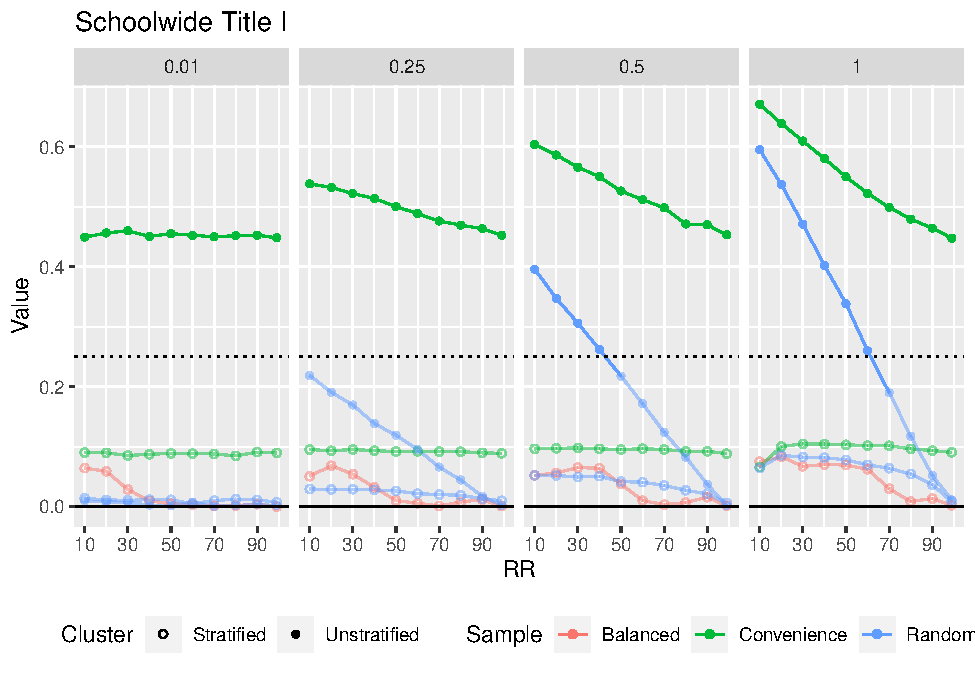
\includegraphics{5---Analysis_files/figure-latex/unnamed-chunk-18-2.pdf} 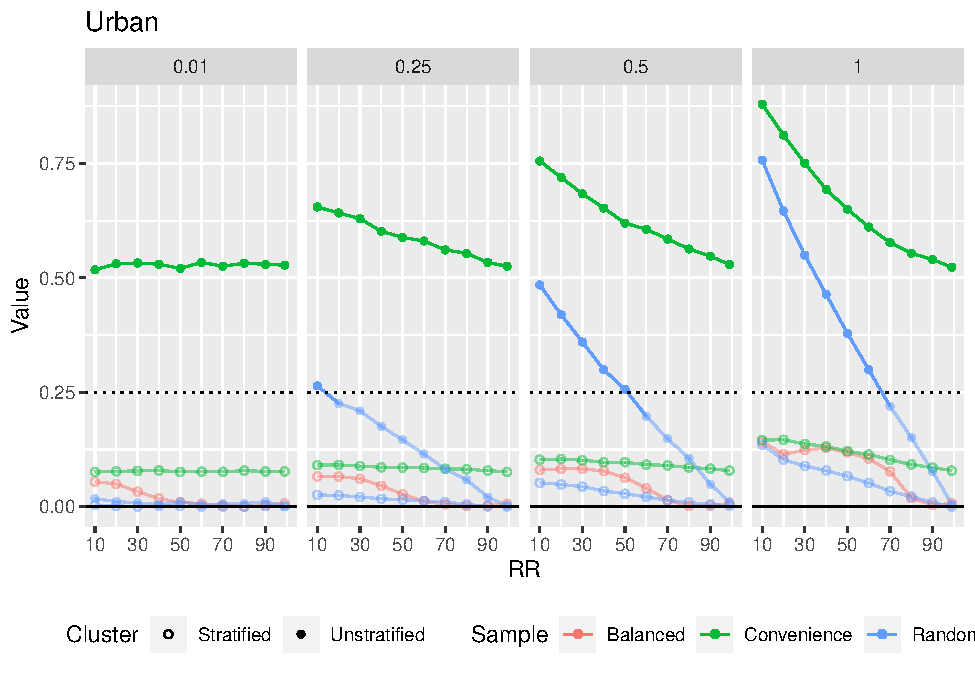
\includegraphics{5---Analysis_files/figure-latex/unnamed-chunk-18-3.pdf}
\#\#\#\# Group 2
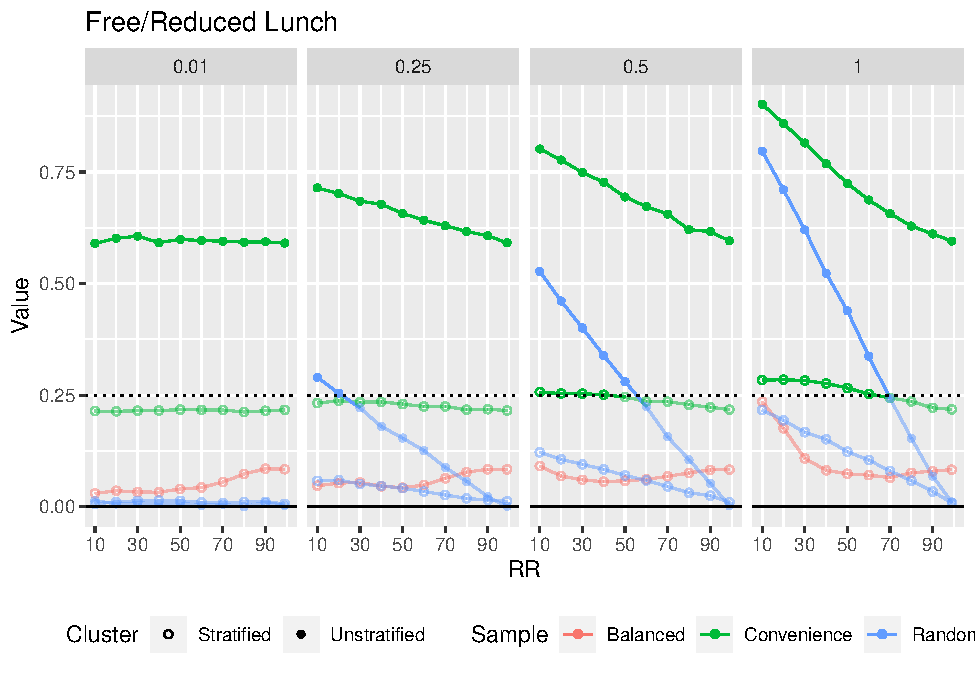
\includegraphics{5---Analysis_files/figure-latex/unnamed-chunk-19-1.pdf} 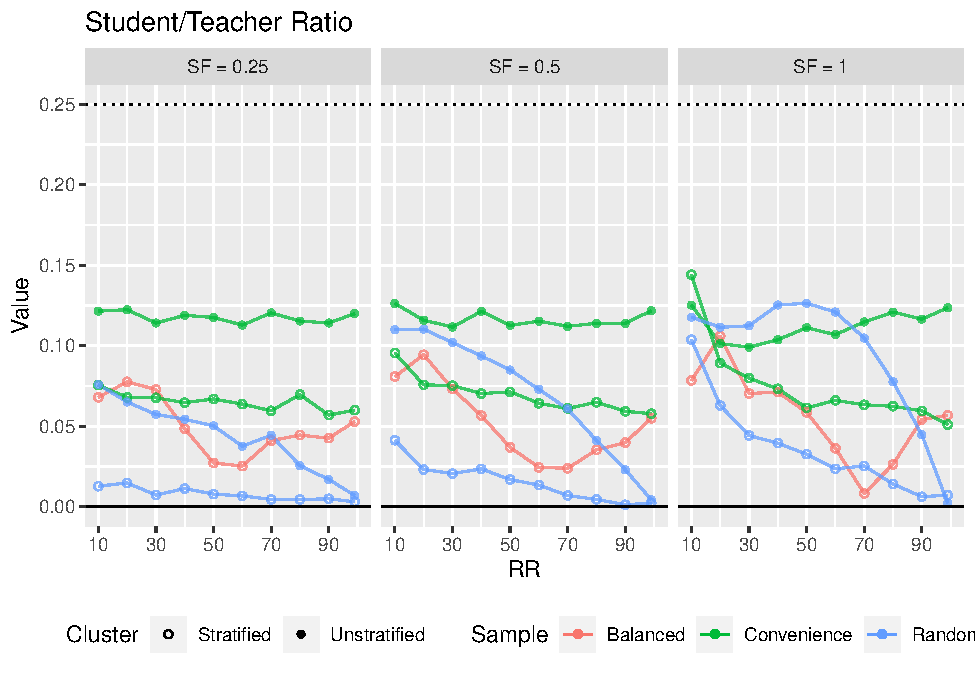
\includegraphics{5---Analysis_files/figure-latex/unnamed-chunk-19-2.pdf} 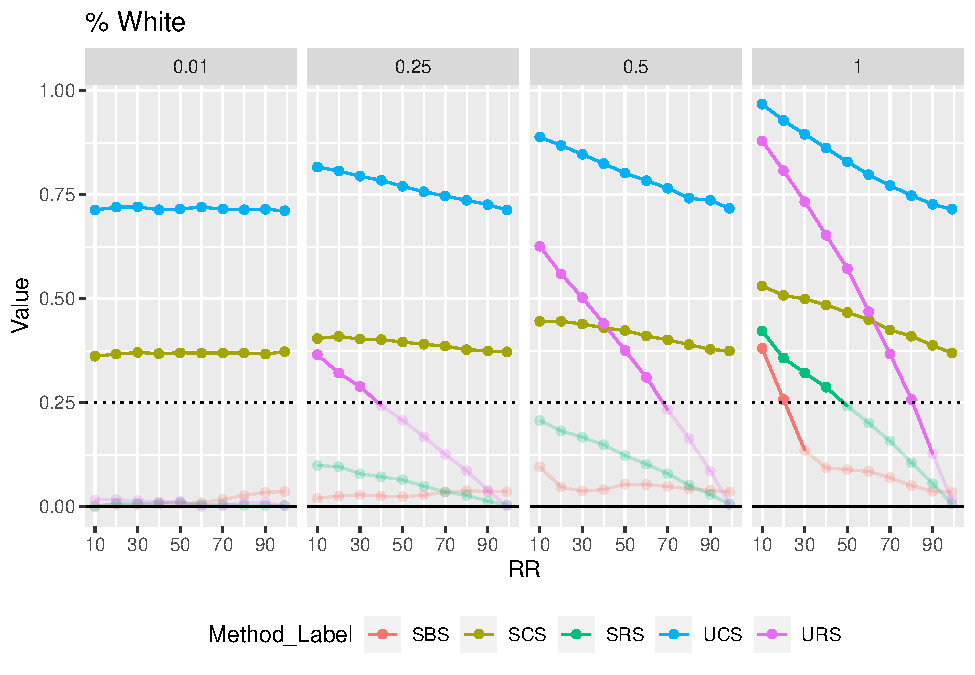
\includegraphics{5---Analysis_files/figure-latex/unnamed-chunk-19-3.pdf} 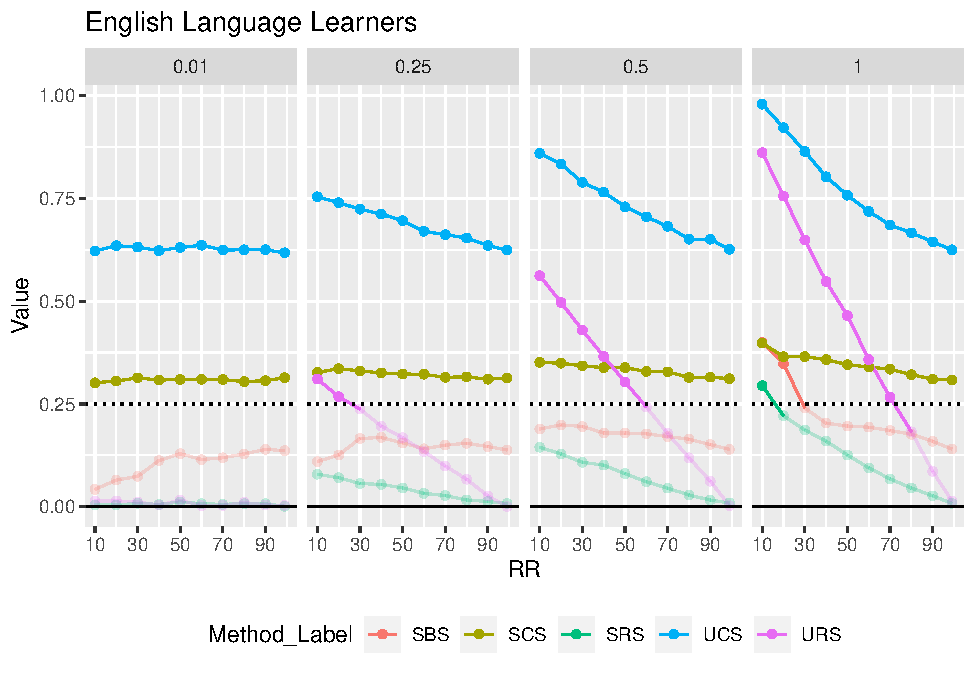
\includegraphics{5---Analysis_files/figure-latex/unnamed-chunk-19-4.pdf} 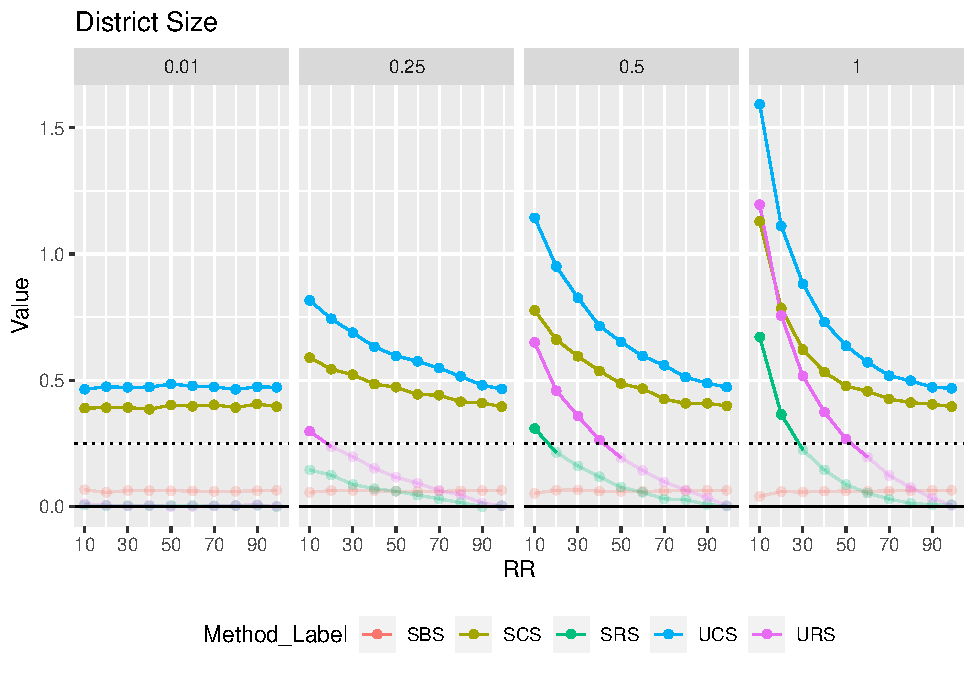
\includegraphics{5---Analysis_files/figure-latex/unnamed-chunk-19-5.pdf}

\hypertarget{group-3}{%
\paragraph{Group 3}\label{group-3}}

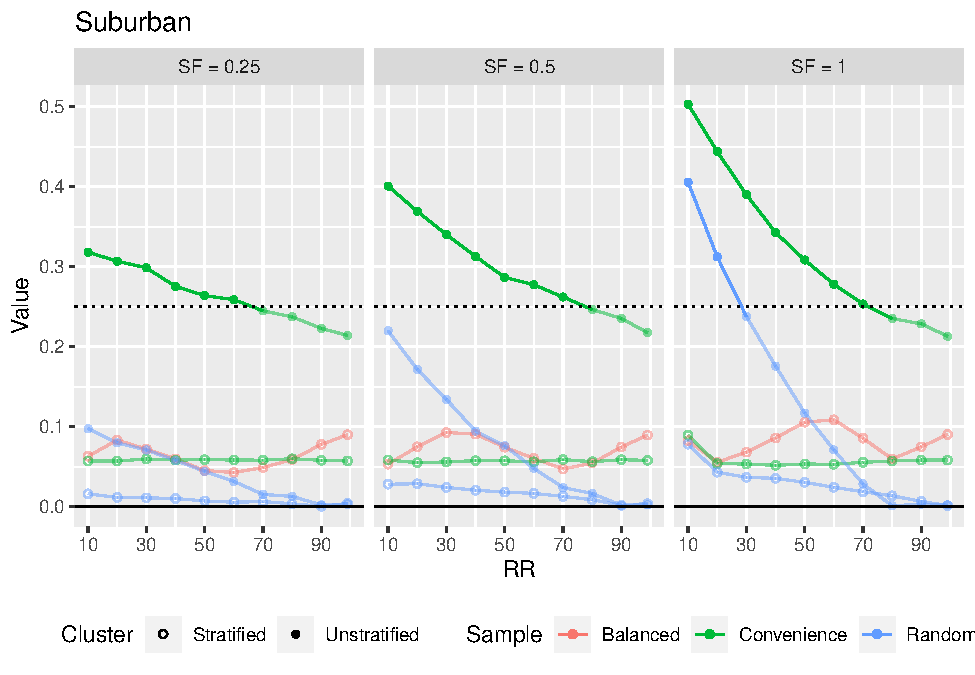
\includegraphics{5---Analysis_files/figure-latex/unnamed-chunk-20-1.pdf} 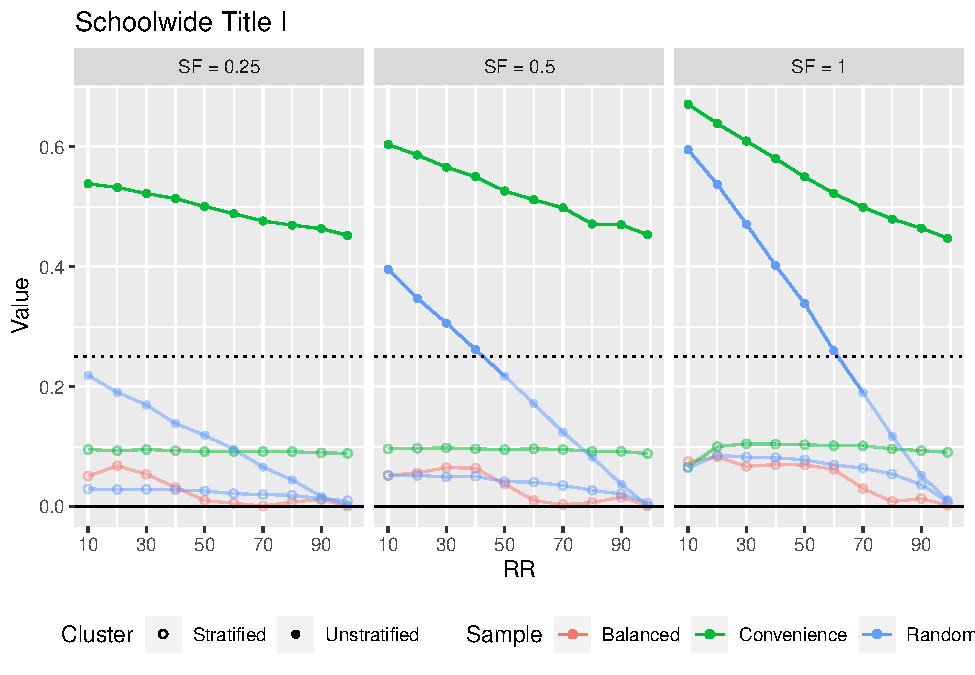
\includegraphics{5---Analysis_files/figure-latex/unnamed-chunk-20-2.pdf} 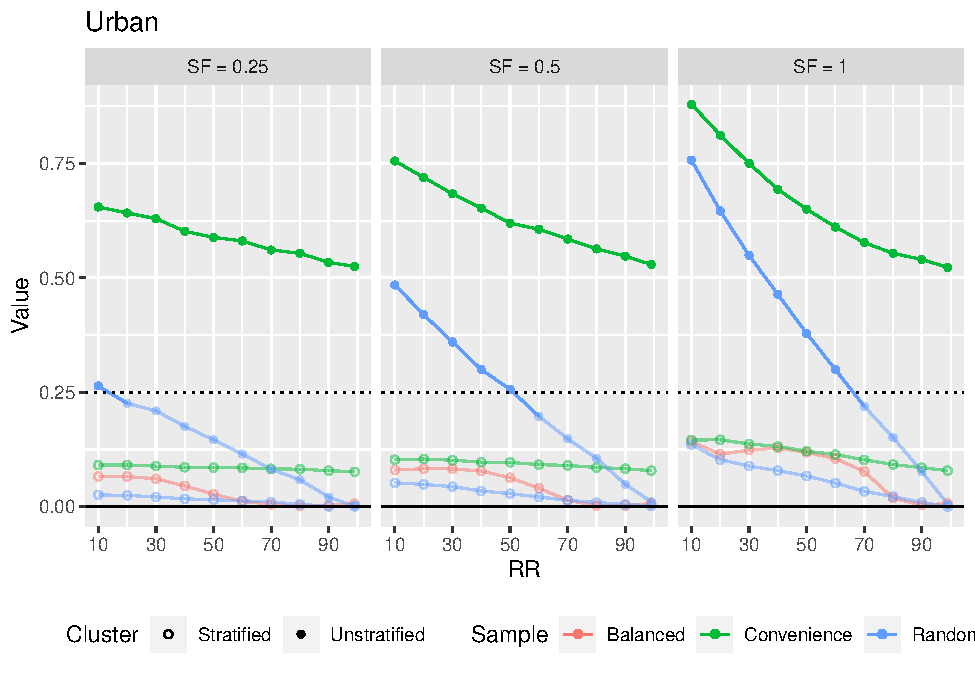
\includegraphics{5---Analysis_files/figure-latex/unnamed-chunk-20-3.pdf}

\hypertarget{group-4}{%
\paragraph{Group 4}\label{group-4}}

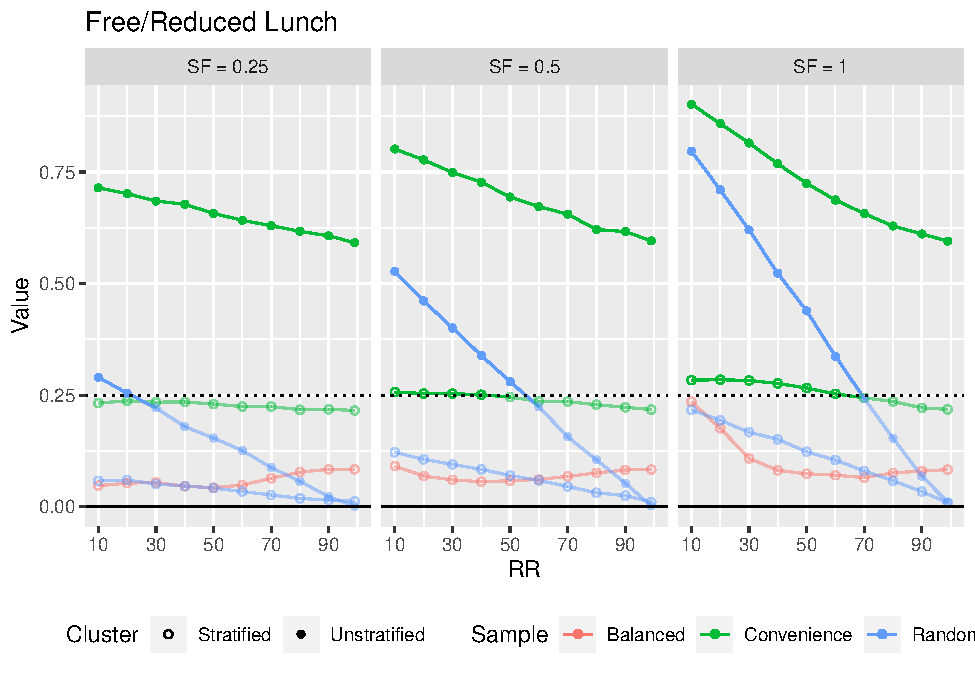
\includegraphics{5---Analysis_files/figure-latex/unnamed-chunk-21-1.pdf} 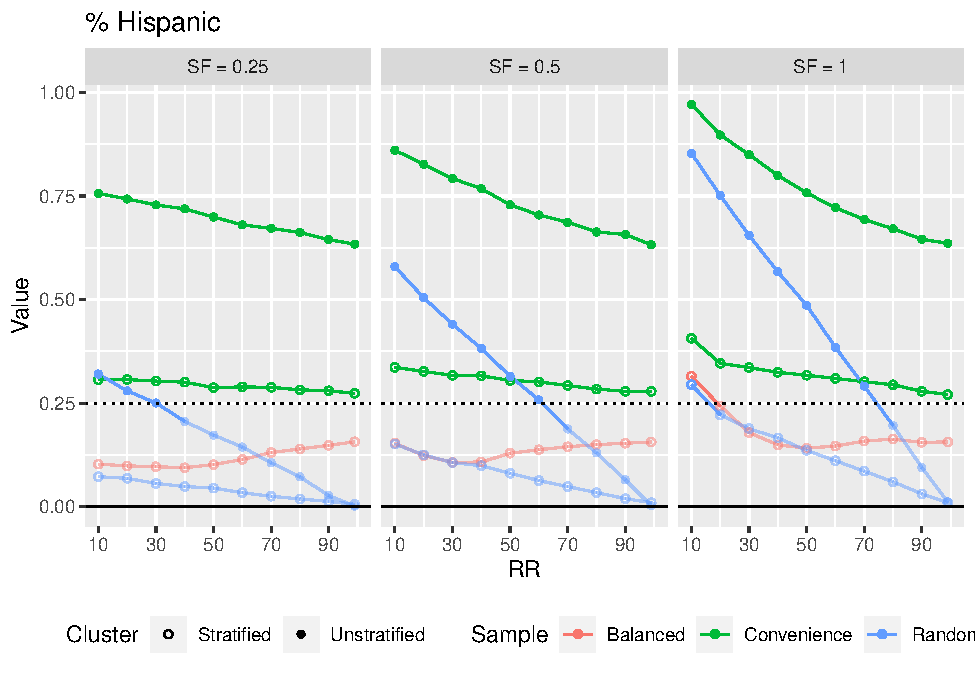
\includegraphics{5---Analysis_files/figure-latex/unnamed-chunk-21-2.pdf}

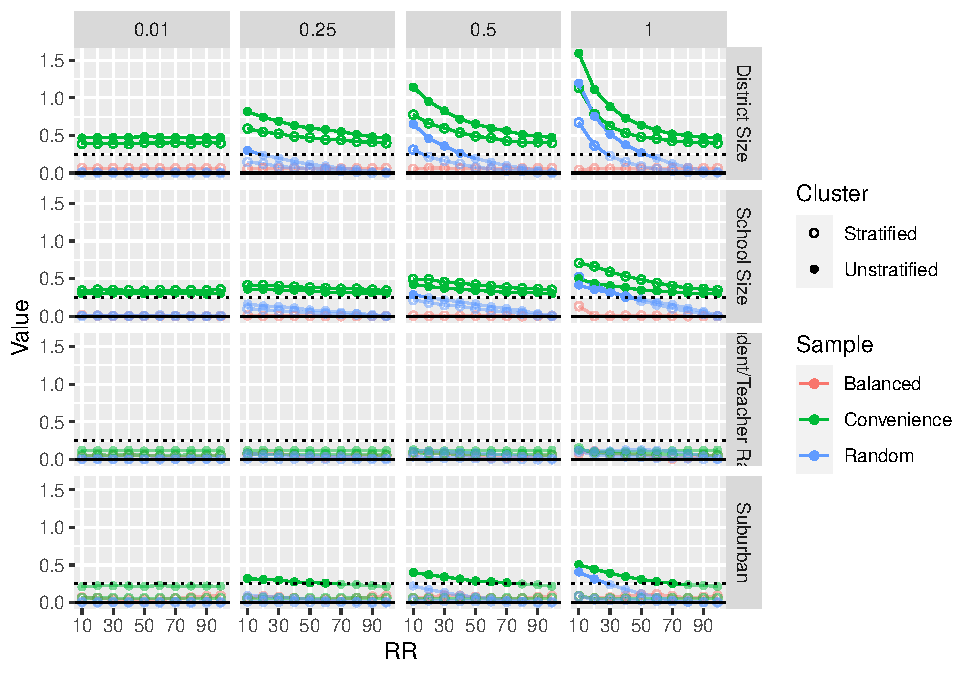
\includegraphics{5---Analysis_files/figure-latex/unnamed-chunk-23-1.pdf}

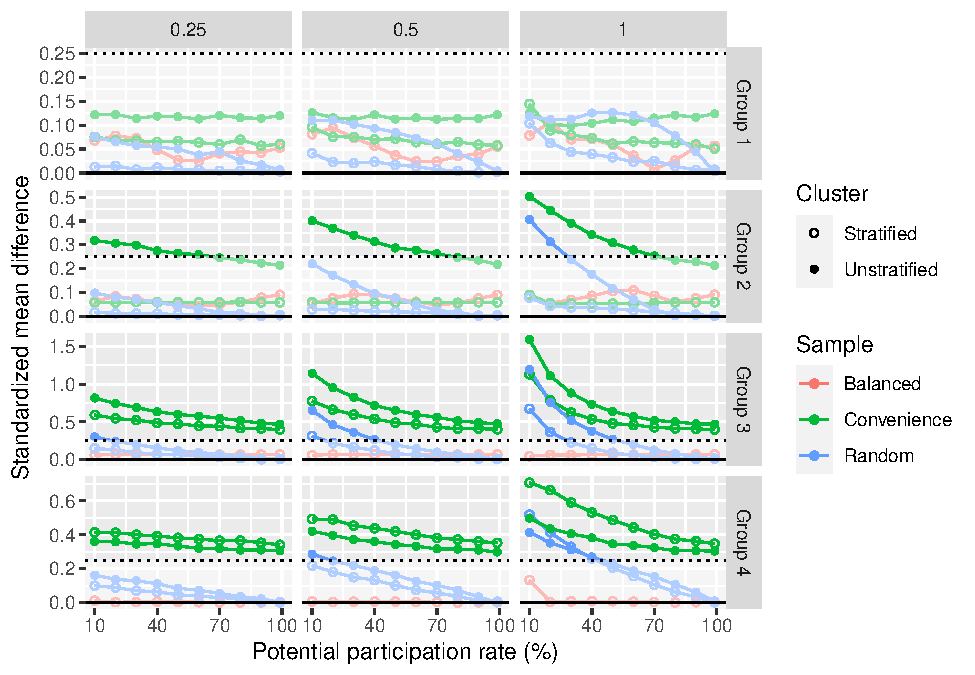
\includegraphics{5---Analysis_files/figure-latex/unnamed-chunk-24-1.pdf}
\#\#\# Examples for presentations

\hypertarget{v-ratio-and-log-odds}{%
\subsubsection{V-ratio and Log odds}\label{v-ratio-and-log-odds}}

\hypertarget{feasibility}{%
\subsection{Feasibility}\label{feasibility}}

\hypertarget{sampling-difficulty}{%
\subsubsection{Sampling Difficulty}\label{sampling-difficulty}}

\begin{figure}
\centering
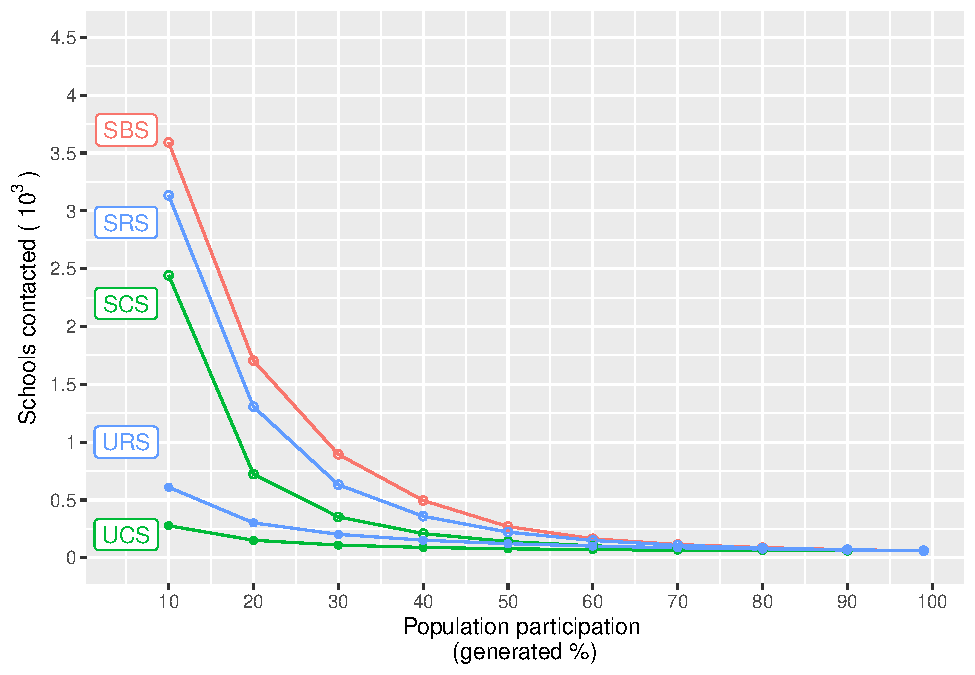
\includegraphics{5---Analysis_files/figure-latex/unnamed-chunk-29-1.pdf}
\caption{\label{fig:unnamed-chunk-29}Schools Contacted}
\end{figure}

\begin{figure}
\centering
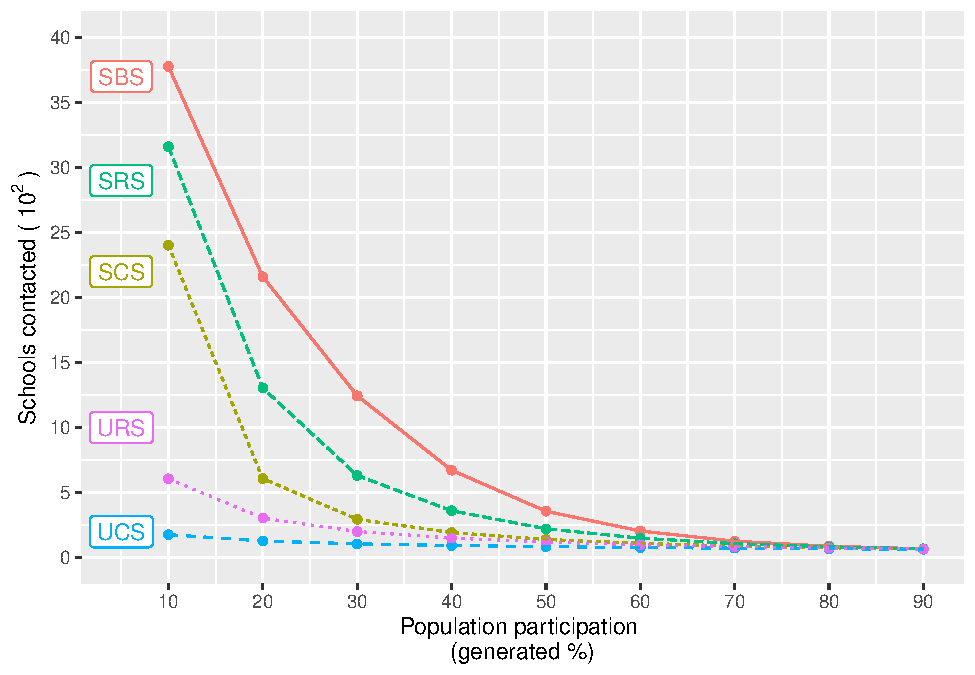
\includegraphics{5---Analysis_files/figure-latex/unnamed-chunk-30-1.pdf}
\caption{\label{fig:unnamed-chunk-30}Sampling response rates}
\end{figure}

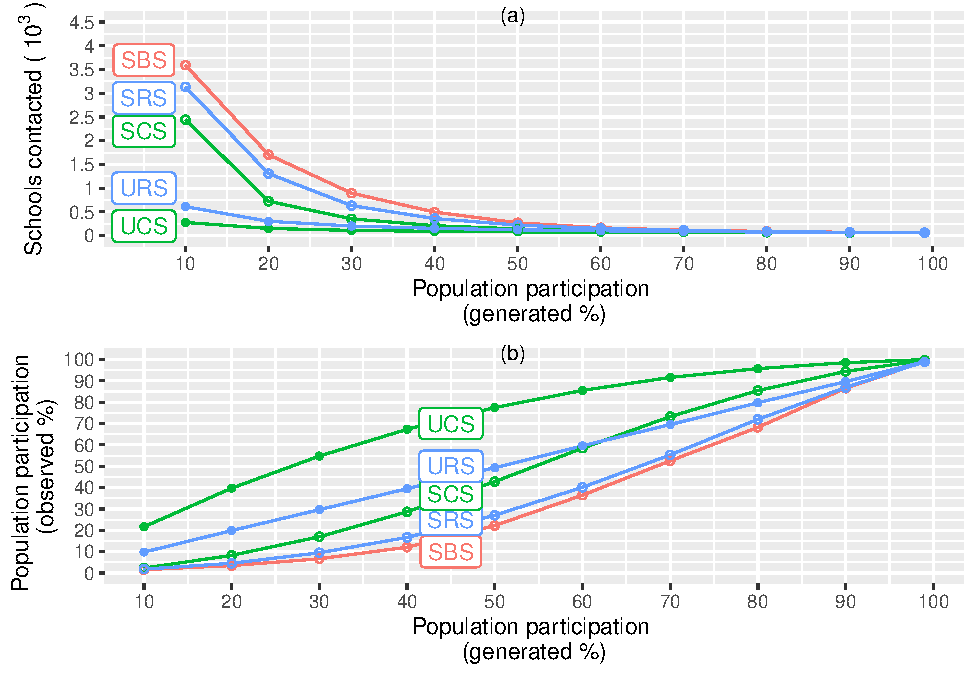
\includegraphics{5---Analysis_files/figure-latex/unnamed-chunk-31-1.pdf}

\hypertarget{relative-performance}{%
\subsubsection{Relative Performance}\label{relative-performance}}

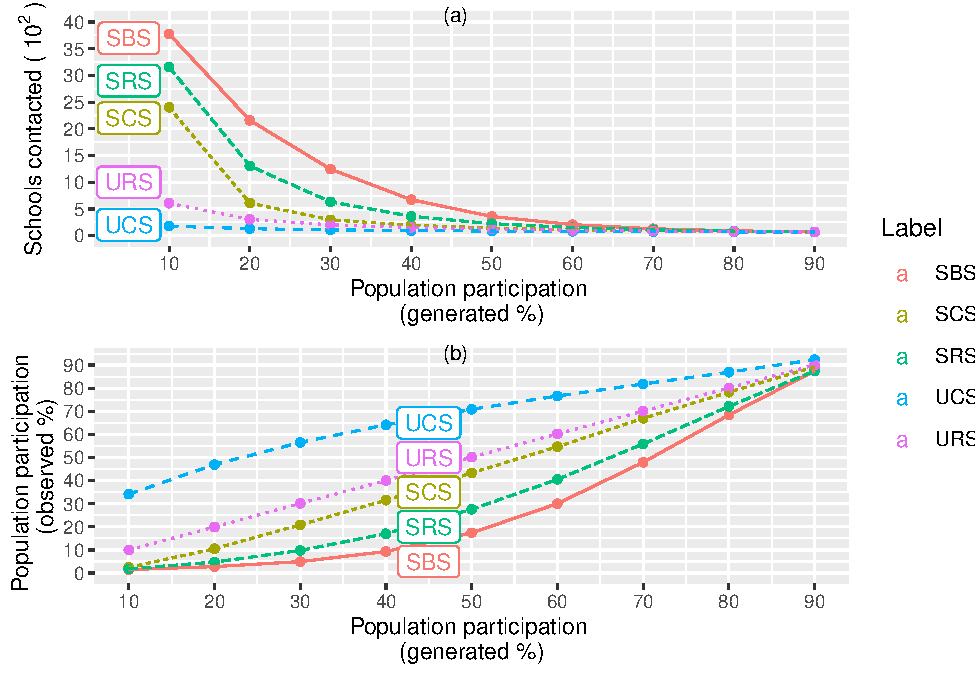
\includegraphics{5---Analysis_files/figure-latex/unnamed-chunk-32-1.pdf}

\hypertarget{gini-plot}{%
\subsubsection{Gini Plot}\label{gini-plot}}

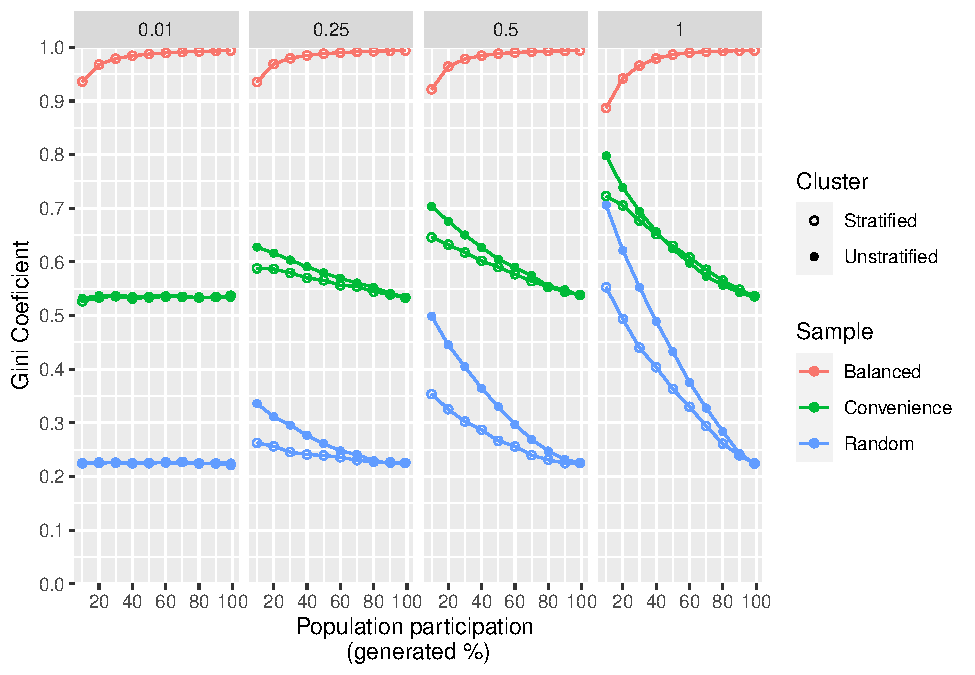
\includegraphics{5---Analysis_files/figure-latex/unnamed-chunk-34-1.pdf}

\hypertarget{a-tibble-22-x-2}{%
\section{A tibble: 22 x 2}\label{a-tibble-22-x-2}}

Vars MB\\
\strut \\
1 tabs 473.73 Mb
2 figs 301.579 Mb
3 results 84.955 Mb
4 df.list 21.411 Mb
5 df.sim 3.027 Mb\\
6 legend 1.161 Mb\\
7 smd.examples.sep 0.214 Mb\\
8 plot\_smd 0.077 Mb\\
9 df.smd.ipsw 0.038 Mb\\
10 get\_quant 0.03 Mb\\
\# \ldots{} with 12 more rows


\end{document}
